\documentclass[10pt,conference,compsocconf]{IEEEtran}

\usepackage{hyperref}
\usepackage{graphicx}	% For figure environment
\usepackage{enumitem}% http://ctan.org/pkg/enumitem
\usepackage[table,xcdraw]{xcolor}
\usepackage{amsfonts} 

\begin{document}
\title{Learning to discover: the Higgs
boson machine learning challenge}

\author{
  Lucas Trognon, Mahammad Ismayilzada, Harold Benoit\\
  \textit{EPFL, Switzerland}
}

\maketitle

\begin{abstract}
This paper reports our work on the Higgs boson machine learning challenge, a high-dimensional classification problem. We have achieved 82\% accuracy with a logistic regression model. Data analysis, feature engineering, and model selection are meticulously written down such that the reader should be able to reproduce our work.
\end{abstract}

\section{Introduction}
The Higgs boson is a famous elementary particle in the Standard Model of particle physics. To make it simple, physicists at CERN would like to detect its existence, and to do so, they smash protons into one another at
high speeds to generate even smaller particles\cite{project_presentation}. The Higgs boson decays rapidly into other particles, so scientists don't observe it directly,
but rather measure its "decay signature". Since many decay
signatures look similar, it is our job to estimate the likelihood that a given event's signature was the result of a
Higgs boson (signal) or some other process/particle (background) given a vector of features representing the decay signatures of a collision event.
\section{Models and Methods}

\subsection{Exploratory Data Analysis and Feature Engineering}


\subsubsection{Data Analysis}

\begin{itemize}
    \item We have at our disposal about 250,000 observations represented with 30 numerical features. About half of the features are primitive raw results, whereas the other half have been derived from these raw features.
    \item The label is defined as "signal" (Boson) or "background" (not Boson).
    \item Variables that are "undefined" take the value -999.0. This value is meaningless and thus it should be treated in the pre-processing such that our models don't interpret this value literally.
    \item Taking a closer look at the original paper \cite{dataset_paper}, these "undefined" values are not random and in fact, systematically missing based on the \textit{PRI\_jet\_num} feature e.g. \textit{PRI\_jet\_leading\_eta} is undefined if \textit{PRI\_jet\_num} = 0. 
    \item Plotting the feature distributions, multiple positively skewed distributions were observed [\ref{fig:skew_fig}].
    \item Furthermore, the \textit{PRI\_jet\_num} feature seems to play a significant role in the behavior of our data. Indeed, it was observed that some features, while discriminating on \textit{PRI\_jet\_num}, experienced significant changes in their distribution. We will come back to this later in our preprocessing.
    
\end{itemize}


\subsubsection{Data Pre-processing}

Data pre-processing is key to good performance in ML. We must try to give our model data that is represented in a meaningful way such that it can accurately capture the structure of the problem and doesn't get caught in the traps of dirty data.
\\

Our pre-processing was done as follows:

\begin{enumerate}
    \item Convert -999 values to NaNs for easier further processing.
    \item For each feature, compute the $\frac{\# \text{of NaNs}}{\text{Total}}$ ratio for each feature. We will call it \textit{nan\_ratio}.
    \item Then based on the specified values of \textit{imputable\_th} and \textit{encodable\_th}, perform the following steps for each feature:
        \begin{itemize}
            \item If $\textit{nan\_ratio} < \textit{imputable\_th}$, the feature is considered as having enough meaningful values to impute the missing values with the median of the feature.
            \item If $\textit{imputable\_th} < \textit{nan\_ratio} < \textit{encodable\_th}$, the feature is considered as having too many missing values to be imputed but not too many such that it is still possibly meaningful. The feature is boolean-encoded i.e. if the value is \textit{NaN} then output 1 else 0.
            \item If $\textit{nan\_ratio} > \textit{encodable\_th }$, the feature is considered as having too many missing values to be useful to the model and it is dropped.
        \end{itemize}
    \item Apply log transformation to the positive features to normalize skewed distributions.
    \item Standardize continuous features to make features with different units comparable to each other.
    \item Add a bias column.
    \item Remove outliers. Here a standardized feature value is considered an outlier if it is outside of the \textit{[-4, 4]} interval.
    \item Switch label encoding from \{-1,1\} to \{0,1\} (for logistic regression only)
    
\end{enumerate}

\hfill


\subsubsection{Feature Engineering}
\begin{enumerate}
    \item The models at our disposal (Linear Regression and Logistic Regression) are all linear models. Since physical processes tend to be highly non-linear, it is vital to augment our features such that the model can capture these complex relationships.
\\

    We define a parameter $\textit{degree}$ which will be a hyper-parameter that will be tuned through grid search and cross-validation. Each continuous feature is, then, polynomially expanded i.e. \begin{equation} x \rightarrow x, ..., x^{\textit{degree}}
    \end{equation} 
    \item Since we observed the fact that the number of jets (\textit{PRI\_jet\_num}) plays a crucial discriminatory role that dictates what features are not relevant (e.g. undefined) for different subsets of the data, we are going to split the dataset into 3 non-overlapping subsets based on this feature i.e. subsets of observations that have 0, 1, and more than 1 jet respectively. Then for each subset, we are going to only retain features that are relevant for it based on \cite{dataset_paper} i.e. when \textit{PRI\_jet\_num} = 0, all jet-related features are not relevant. We will use these 3 subsets of data to train 3 separate models. At prediction time, a given vector of features will be predicted using the model corresponding to its number of jets.
\end{enumerate}


\subsection{Model Selection and Hyperparameter Tuning}

\subsubsection{Model Selection}

We have 6 models (Least Squares using Normal Equations, Least Squares using (Stochastic) Gradient Descent, Ridge Regression, Logistic Regression and $\mathbb{L}_2$ Regularized Logistic Regression) to choose from. To choose the best model, we ran each model under different conditions and reported the 5-fold cross-validated accuracy for comparison. The conditions steadily increase in feature engineering complexity:
\begin{enumerate}[label=\Roman*]
    \item On unprocessed raw data.
    \item On preprocessed data, where all features that have at least one NaN value are imputed with the median (i.e. \textit{imputable\_th}=1, \textit{encodable\_th}=0).
    \item On preprocessed data, where all features that have at least one NaN value are boolean-encoded (i.e. \textit{encodable\_th}=1, \textit{imputable\_th}=0).
    \item On preprocessed data, where features that have at most 30\% of their values as NaN value are imputed. Features that have between 30\% and 70\% of their values as NaN values are boolean-encoded. All other features are dropped from the dataset (i.e. \textit{encodable\_th}=0.3, \textit{imputable\_th}=0.7).
    \item Take the option out of \{I, II, III, IV\} that yielded the best accuracy and polynomially expand the continuous features.
    \item Same steps as V, but the data is now split into 3 datasets based on the number of jets, as described previously. 3 separate models are trained. The reported accuracy is the weighted average accuracy of the 3 models. The weight is the number of rows of each dataset.
\end{enumerate}

To give each model its best chance to perform, the reported accuracy is the best 5-fold cross validated result over the grid search over these range of parameters (when applicable for the given algorithm) :

\begin{itemize}
    \item $\textit{degree}$ = $\{1, 2, 3, 4\}$
    \item $\lambda$ = $\{0.01, 0.1\}$
    \item $\gamma$ = $\{0.01, 0.1\}$
\end{itemize}

\hfill


The results from this model selection are reported in Table \ref{tab:my-table}.


\subsubsection{Hyper-parameter selection}

After choosing  $\mathbb{L}_2$ regularized logistic regression as our model of choice, we decided to do some hyper-parameter fine-tuning to get the best model possible.
We did a grid-search over these range of parameters:
\begin{itemize}
    \item $\textit{degree}$ = $\{1, 2, 3, 4\}$
    \item $\lambda$ = $\{10^{-3}, 10^{-2}, 10^{-1}, 1\}$
    \item $\gamma$ = $\{0.01, 0.1\}$
\end{itemize}
\hfill

For each combination of these parameters, we ran k-fold cross-validation with $K=5$ to accurately compute the loss of the model. Each model was optimized using gradient descent with 1000 iterations. Once we fine-tuned the hyperparameters, we ran our model with tuned hyperparameter values for 3000 iterations to reduce the loss further and increase accuracy.

Our final hyperparameters are:

\begin{itemize}
    \item  $\textit{degree}$ = 3, $\lambda = 0.001$, $\gamma = 0.1$ 
    \item \textit{imputable\_th}= 1, \textit{encodable\_th}= 0
\end{itemize}

\section{Results}

As can be seen from Table \ref{tab:my-table}, our best models were the logistic regression models. Our peak accuracy, after fine-tuning, was 82\%.

Additionally, our feature engineering proved to be useful as every step increased the accuracy for every model. Polynomial expansion seems to be necessary to capture non-linearities as \textit{degree} = 3 was chosen by the cross-validation.

\section{Discussion}

Logistic regression is a simple model. Thus, it has interpretability. But its simplicity may also be its weakness as it means that we need to rely on heuristics, such as polynomial expansion, to capture non-linear relationships.

We could have used neural nets such that we learn the features from the data in the same way as we learn the weights of the linear classifier, but we currently lack the knowledge to apply neural nets to this problem.

As of today, neural nets seem to be the option of choice. It would be interesting to see if better accuracy would be reached using them.

\section{Summary}
We have successfully applied Machine Learning to classify particles' decay signature as originating from the Higgs Boson. We have obtained 82\% accuracy on both training and the test set. Thanks to the interpretability of our model, it is possible to evaluate which measurement is significant to the Boson signature. Physicists may find it insightful.

\section*{Acknowledgements}
The authors thank the EPFL ML course for such an interesting project.

\begin{table}[]
\centering
\begin{tabular}{
>{\columncolor[HTML]{EFEFEF}}l |
>{\columncolor[HTML]{FFFFFF}}l |
>{\columncolor[HTML]{FFFFFF}}l |
>{\columncolor[HTML]{FFFFFF}}l |
>{\columncolor[HTML]{FFFFFF}}l |
>{\columncolor[HTML]{FFFFFF}}l |
>{\columncolor[HTML]{FFFFFF}}l |}
\cline{2-7}
\cellcolor[HTML]{FFFFFF}                          & \cellcolor[HTML]{EFEFEF}OLS & \cellcolor[HTML]{EFEFEF}LS\_GD & \cellcolor[HTML]{EFEFEF}LS\_SGD & \cellcolor[HTML]{EFEFEF}Ridge & \cellcolor[HTML]{EFEFEF}Log & \cellcolor[HTML]{EFEFEF}Reg\_Log \\ \hline
\multicolumn{1}{|l|}{\cellcolor[HTML]{EFEFEF}I}   & 74.43                       & 0.0                            & 0.0                             & 74.42                         & 59.74                       & 63.67                            \\ \hline
\multicolumn{1}{|l|}{\cellcolor[HTML]{EFEFEF}II}  & 76.44                       & 76.43                          & 72.55                           & 76.44                         & 76.21                       & 75.66                            \\ \hline
\multicolumn{1}{|l|}{\cellcolor[HTML]{EFEFEF}III} & 0.0                         & 75.19                          & 71.50                           & 75.14                         & 75.50                       & 74.73                            \\ \hline
\multicolumn{1}{|l|}{\cellcolor[HTML]{EFEFEF}IV}  & 70.99                       & 75.41                          & 72.93                           & 75.44                         & 75.27                       & 74.53                            \\ \hline
\multicolumn{1}{|l|}{\cellcolor[HTML]{EFEFEF}V}   & 0.0                         & 76.38                          & 72.93                           & 79.87                         & 81.40                       & 80.93                            \\ \hline
\multicolumn{1}{|l|}{\cellcolor[HTML]{EFEFEF}VI}  & 76.82                       & 76.78                          & 73.72                           & 80.79                         & 81.85                       & 81.71                            \\ \hline
\end{tabular}
\caption{Comparison of the 6 models accuracies (\%) under different conditions. A value of 0.0 means that the algorithm wasn't able to converge.}
\label{tab:my-table}
\end{table}

\begin{figure}
    \centering
    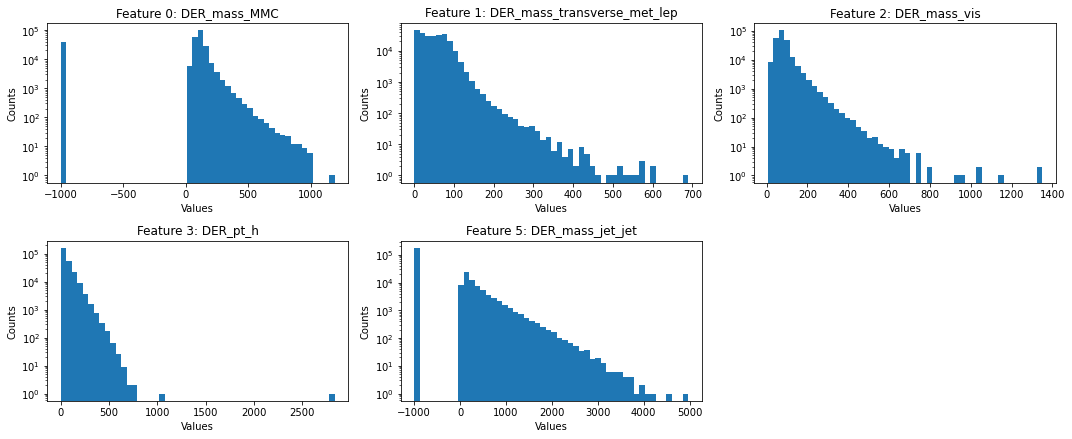
\includegraphics[scale = 0.45]{feature_distribution.png}
    \caption{Feature distribution of the first features in the dataset. The Y axis is in log scale. This plot is meant to showcase the tendency for our dataset to have positively-skewed distributions.}
    \label{fig:skew_fig}
\end{figure}

\bibliographystyle{IEEEtran}
\bibliography{literature}
\end{document}
